\chapter{Evaluation} \label{evaluation}

\section{Overview}

This chapter evaluates the photorealistic scene reconstruction pipeline. The pipeline is divided into two primary stages: post-processing the dataset and generating a Gaussian splat model. For testing the image post-processing script, I created a scene with challenging conditions, including high angular speeds and overexposure, to evaluate the script's ability to filter out unsuitable images. A scene recorded by the robot was used to test the Gaussian splatting and assess the 3D reconstruction quality. 

\section{Image Post-Processing Script}

To assess the effectiveness of the post-processing script, I created a dataset with simulated challenging conditions by making rapid movements and positioning a flashlight near the camera. These actions mimicked high angular speeds and overexposure, aiming to introduce blurry and overexposed frames into the dataset. Figure~\ref{fig:keyframes_before_process} shows the saved keyframe images before running the script.

\FloatBarrier
\begin{figure}[htbp]
	\centering
	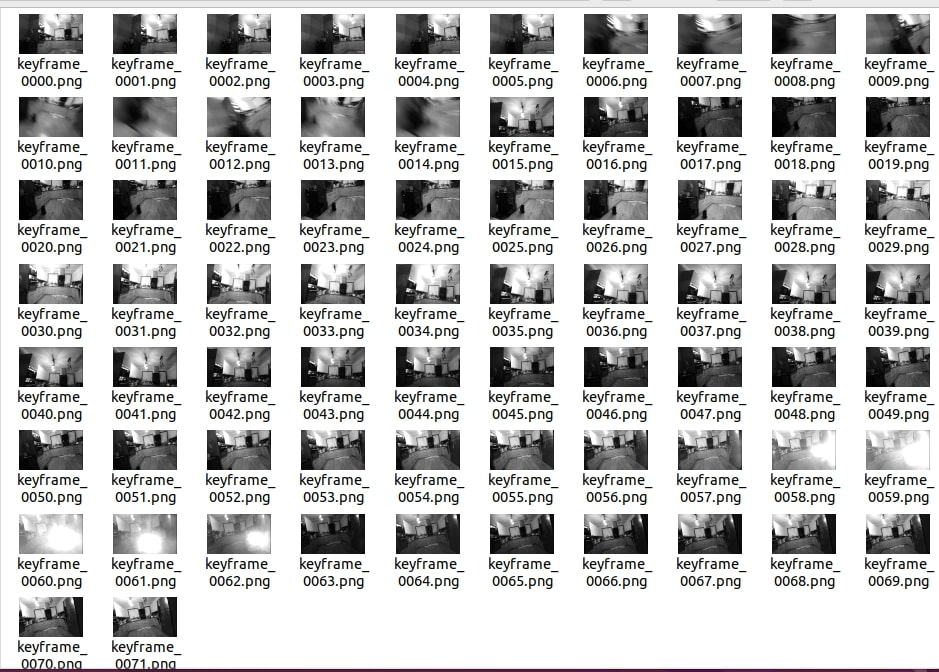
\includegraphics[width=150mm, keepaspectratio]{figures_jpg/keyframes_before_process.jpg}
	\caption{Saved images from mapping by the \textit{keyframe\_saver} node before processing}
	\label{fig:keyframes_before_process}
\end{figure}
\FloatBarrier

After running the script, which detected and removed blurry or overexposed frames, the processed image set can be seen in Figure~\ref{fig:keyframes_after_process}. The script’s output, detailing deletions and renamings, is shown in Figure~\ref{fig:image_process_script_output}. Examples of detected blurry and overexposed images that the script correctly flagged for deletion are displayed in Figure~\ref{fig:blurry_overexposed_example}.

\FloatBarrier
\begin{figure}[htbp]
	\centering
	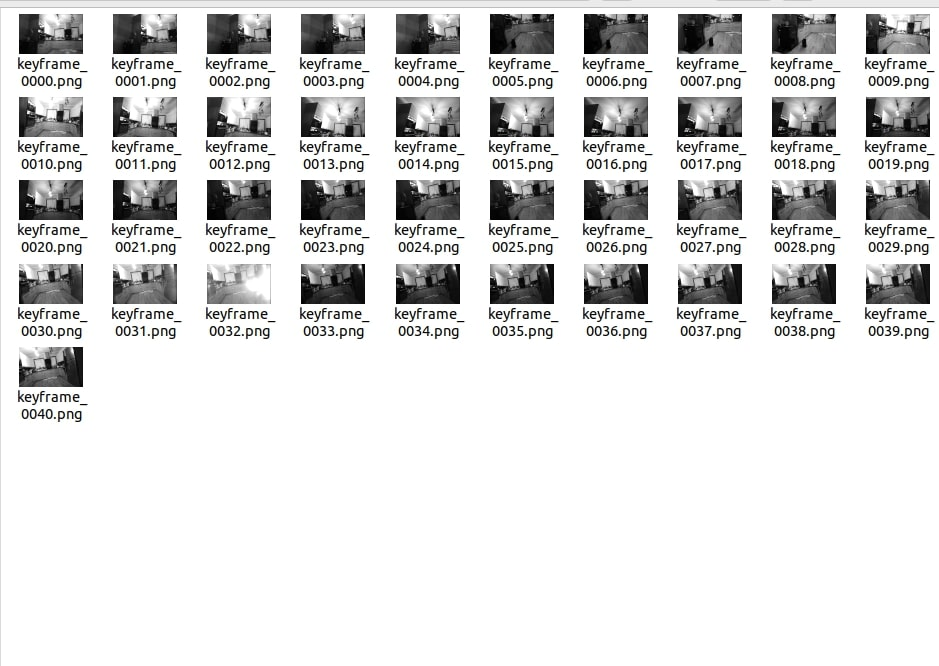
\includegraphics[width=150mm, keepaspectratio]{figures_jpg/keyframes_after_process.jpg}
	\caption{Remaining images after running the post-processing script}
	\label{fig:keyframes_after_process}
\end{figure}

\begin{figure}[htbp]
	\centering
	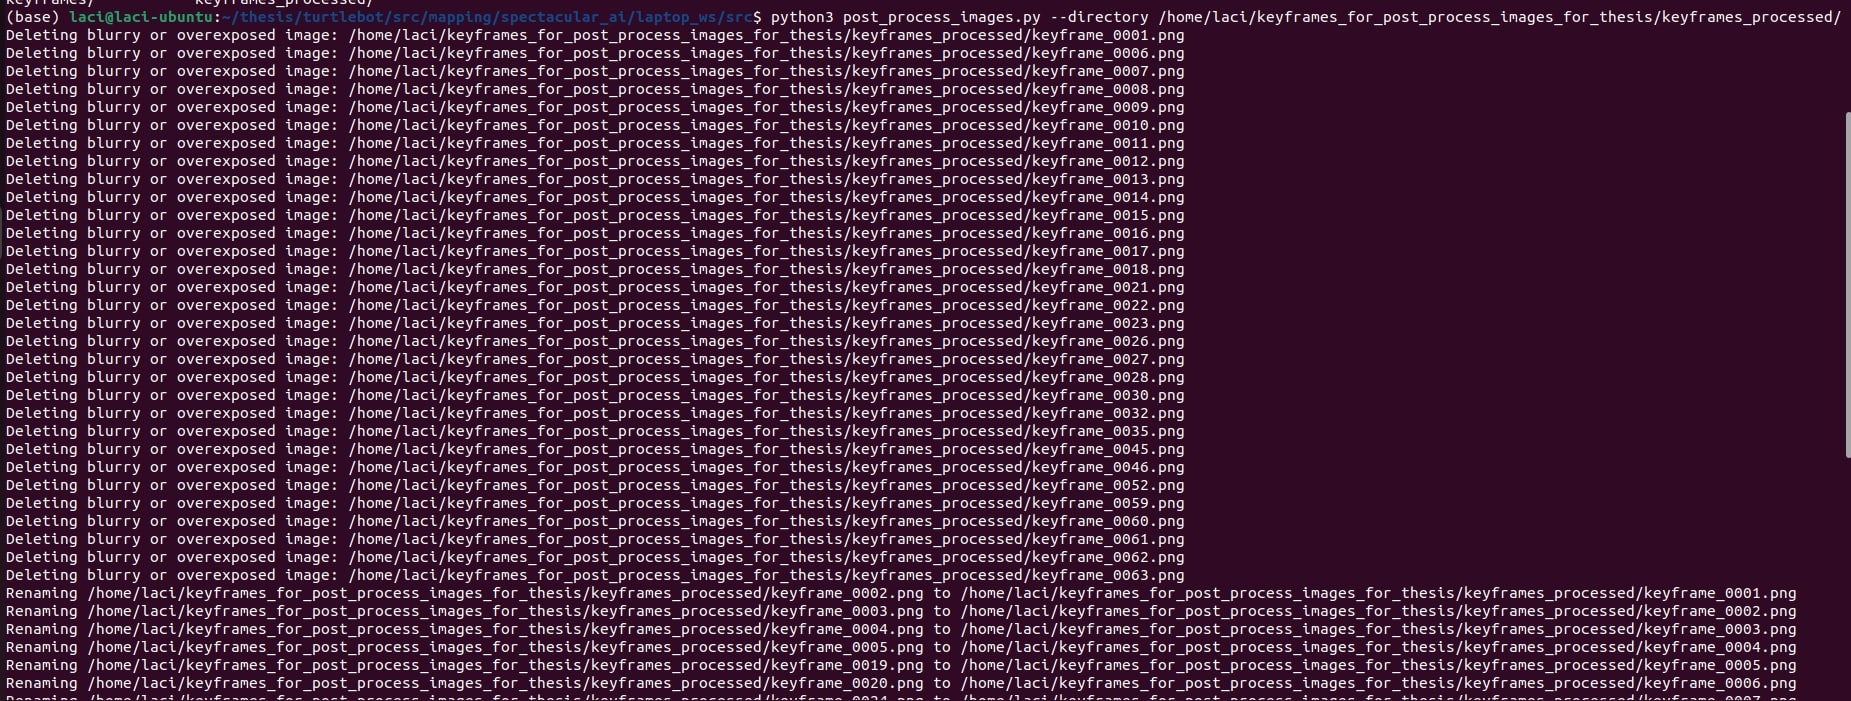
\includegraphics[width=150mm, keepaspectratio]{figures_jpg/process_script_output.jpg}
	\caption{Terminal output of the post-processing script}
	\label{fig:image_process_script_output}
\end{figure}


\begin{figure}[htbp]
	\centering
	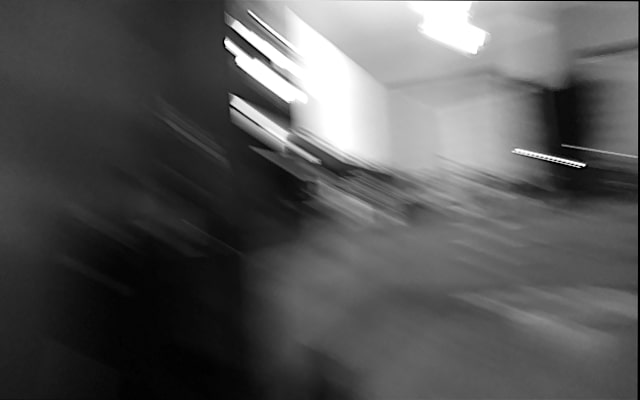
\includegraphics[width=67mm, keepaspectratio]{figures_jpg/example_for_blurry.jpg}\hspace{1cm}
	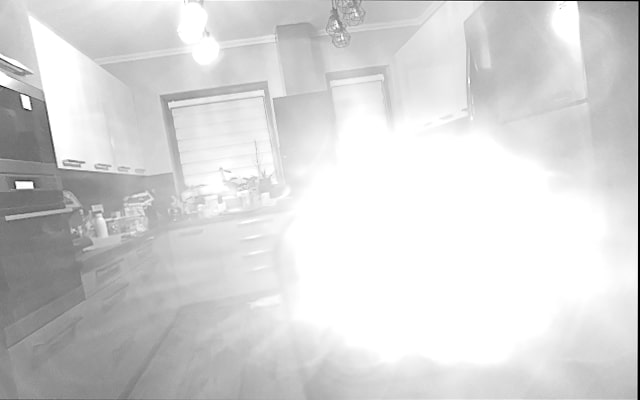
\includegraphics[width=67mm, keepaspectratio]{figures_jpg/example_for_overexposed.jpg}\\\vspace{5mm}
	\caption{Examples of blurry (left) and overexposed (right) images successfully detected and deleted by the script}
	\label{fig:blurry_overexposed_example}
\end{figure}
\FloatBarrier

I would like to note that I ran the dataset post-processing script without including the JSON files that define the poses for the keyframes. This ensures that no additional files appear in the folder shown in the figures, making the contents more straightforward and easier to interpret.

\section{Coordinate Transformations}

The output of the node that collects images and keyframe poses is shown in Figure~\ref{fig:mapping_keyframe_folder}. For each image, a corresponding JSON file is generated, containing the position and orientation of the keyframe where the image was captured. An example of such a pose file for \verb|keyframe_0012| is presented in Figure~\ref{fig:mapping_pose_json}. The images and their associated pose files share the same filename, differing only in their file extensions.

\begin{figure}[htbp]
	\centering
	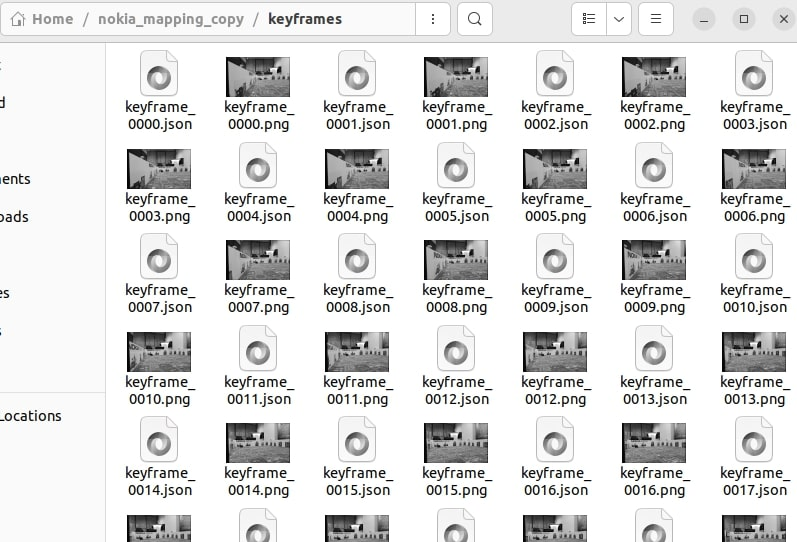
\includegraphics[width=150mm, keepaspectratio]{figures_jpg/mapping_keyframe_folder.jpg}
	\caption{Keyframe images and saved poses}
	\label{fig:mapping_keyframe_folder}
\end{figure}

\begin{figure}[htbp]
	\centering
	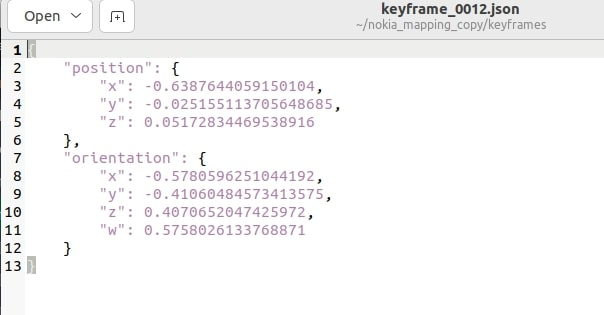
\includegraphics[width=150mm, keepaspectratio]{figures_jpg/mapping_pose_json.jpg}
	\caption{Example for pose JSON file}
	\label{fig:mapping_pose_json}
\end{figure}

Using the collected keyframes and camera intrinsic parameters, I executed my script to prepare the dataset for generating a Gaussian splat. The script processes the data, transforms the point cloud, and outputs the necessary files for the pipeline. A snapshot of the script's execution, including the progress updates for the point cloud transformation, is shown in Figure~\ref{fig:create_splatfacto_script_cli}.

\begin{figure}[htbp]
	\centering
	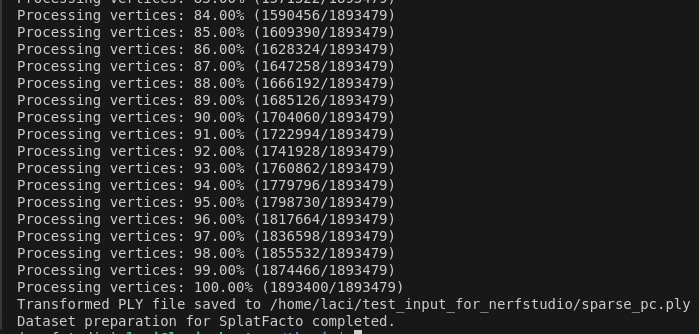
\includegraphics[width=150mm, keepaspectratio]{figures_jpg/create_splatfacto_script_cli.jpg}
	\caption{Output of the script}
	\label{fig:create_splatfacto_script_cli}
\end{figure}

The folder structure generated by the script is depicted in Figure~\ref{fig:nerfstudio_input_by_my_script}. This structure includes a folder containing the keyframe images, a transformed point cloud file, and a \verb|transforms.json| file. The \verb|transforms.json| file encodes the transformation matrices and camera intrinsics corresponding to each image's pose. A snippet of this file for \verb|keyframe_0012| is shown in Figure~\ref{fig:transforms_json}.
\begin{figure}[htbp]
	\centering
	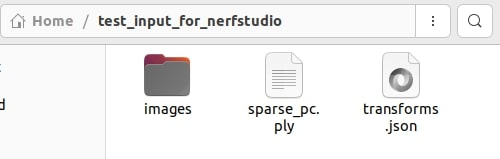
\includegraphics[width=150mm, keepaspectratio]{figures_jpg/nerfstudio_input_by_my_script.jpg}
	\caption{Created input for NeRFstudio by the script}
	\label{fig:nerfstudio_input_by_my_script}
\end{figure}

\begin{figure}[htbp]
	\centering
	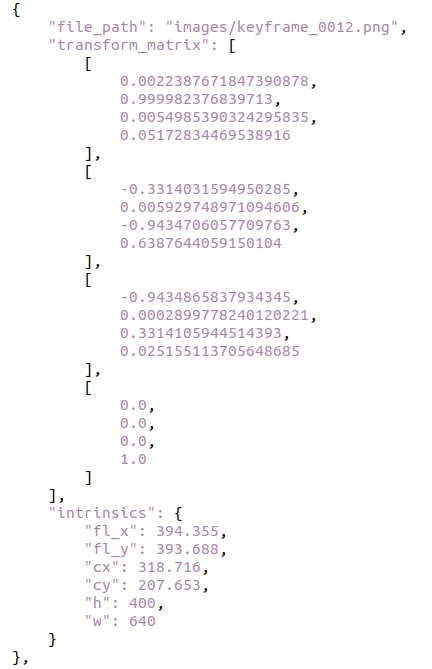
\includegraphics[width=150mm, keepaspectratio]{figures_jpg/transforms_json.jpg}
	\caption{Created transforms.json file}
	\label{fig:transforms_json}
\end{figure}

\FloatBarrier
\section{Gaussian Splatting}

% To evaluate the Gaussian splatting capabilities, I recorded a scene with an old microscope, positioned centrally in a controlled setting. After running the post-processing script to filter the images, I trained the \verb|splatfacto| model on the processed dataset. Figure~\ref{fig:spai_gsplat} displays the reconstructed splat.

% \begin{figure}[htbp]
% 	\centering
% 	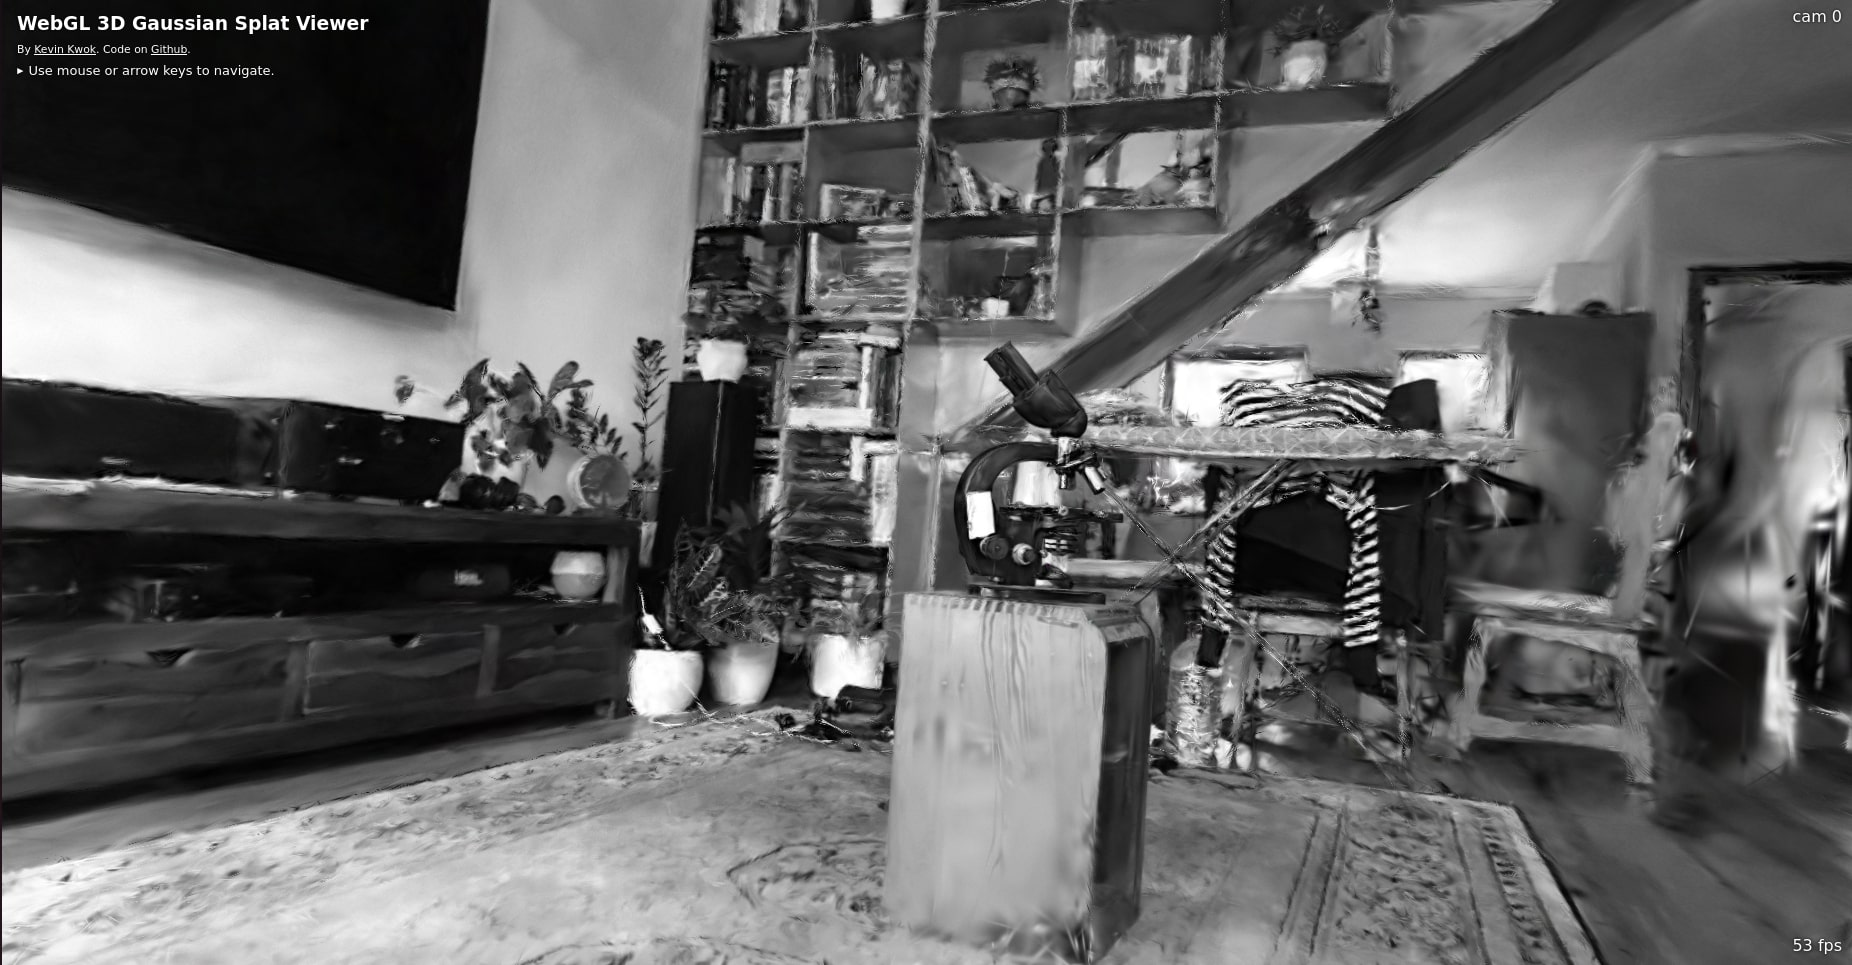
\includegraphics[width=150mm, keepaspectratio]{figures_jpg/spai_gsplat_splatfacto_good.jpg}
% 	\caption{Reconstructed microscope scene using the \textit{splatfacto} model}
% 	\label{fig:spai_gsplat}
% \end{figure}

% TODO: write more about these images
% TODO: compare our results with colmap's estimated poses and pointcloud, here we can write about the noisy pointcloud

To evaluate the capabilities of my pipeline and Gaussian splatting we used the robot in the Nokia office, we drove inside a rectangular area with it, with my mapping node started. We started the keyframe saver and the pointcloud saver nodes on the laptop as well, to be able to capture the images, their keyframes' poses and pointcloud while driving around. Then, after the image post-processing and running the dataset preparator script, we trained the \verb|splatfacto| model. The result can be observed on Figure~\ref{fig:nokia_splatfacto_ours_1} and Figure~\ref{fig:nokia_splatfacto_ours_2}. It can be seen that the created scene is suboptimal, it has critical issues. There are some unique parts in the scene that can be recognised but this is not the result we wanted. I investigated the problem and the following conclusions can be drawn:
\begin{itemize}
    \item The images' quality is good enough for training the model.
    \item The poses are accurate: we measured the distance and the rotation between distant keyframes ourselves and the poses we get from the camera are accurate.
    \item The transformations are checked, during the training process we are able to inspect the trajectory of the keyframes in the viser, and they reflect reality. It is possible to display the pointcloud during training too, with this functionality we could check the alignment of the poses and the pointcloud. It can be seen on Figure~\ref{fig:trajectory_and_pointcloud} and Figure~\ref{fig:pointcloud_debug} that the poses and the pointcloud align well, they show the exact same corner.
    \item I checked the pointcloud, and I realised that the root cause of the misalignments of reality was caused by that. As it can be inspected on Figure~\ref{fig:pointcloud_debug} there are numerous points added to the cloud that are not present in reality, they appear as a noise and corrupt the reconstruction. Gaussian splatting is very sensitive to this kind of noise because it tries to fit a Gaussian to each point, in other words, every point in the cloud will represent a surface in the splat (even the noise). The other problem is that there is a bump in the floor and it causes some points which represent the floor to be slightly tilted, this can be seen on Figure~\ref{fig:pointcloud_debug1}.
\end{itemize}


\begin{figure}[htbp]
	\centering
	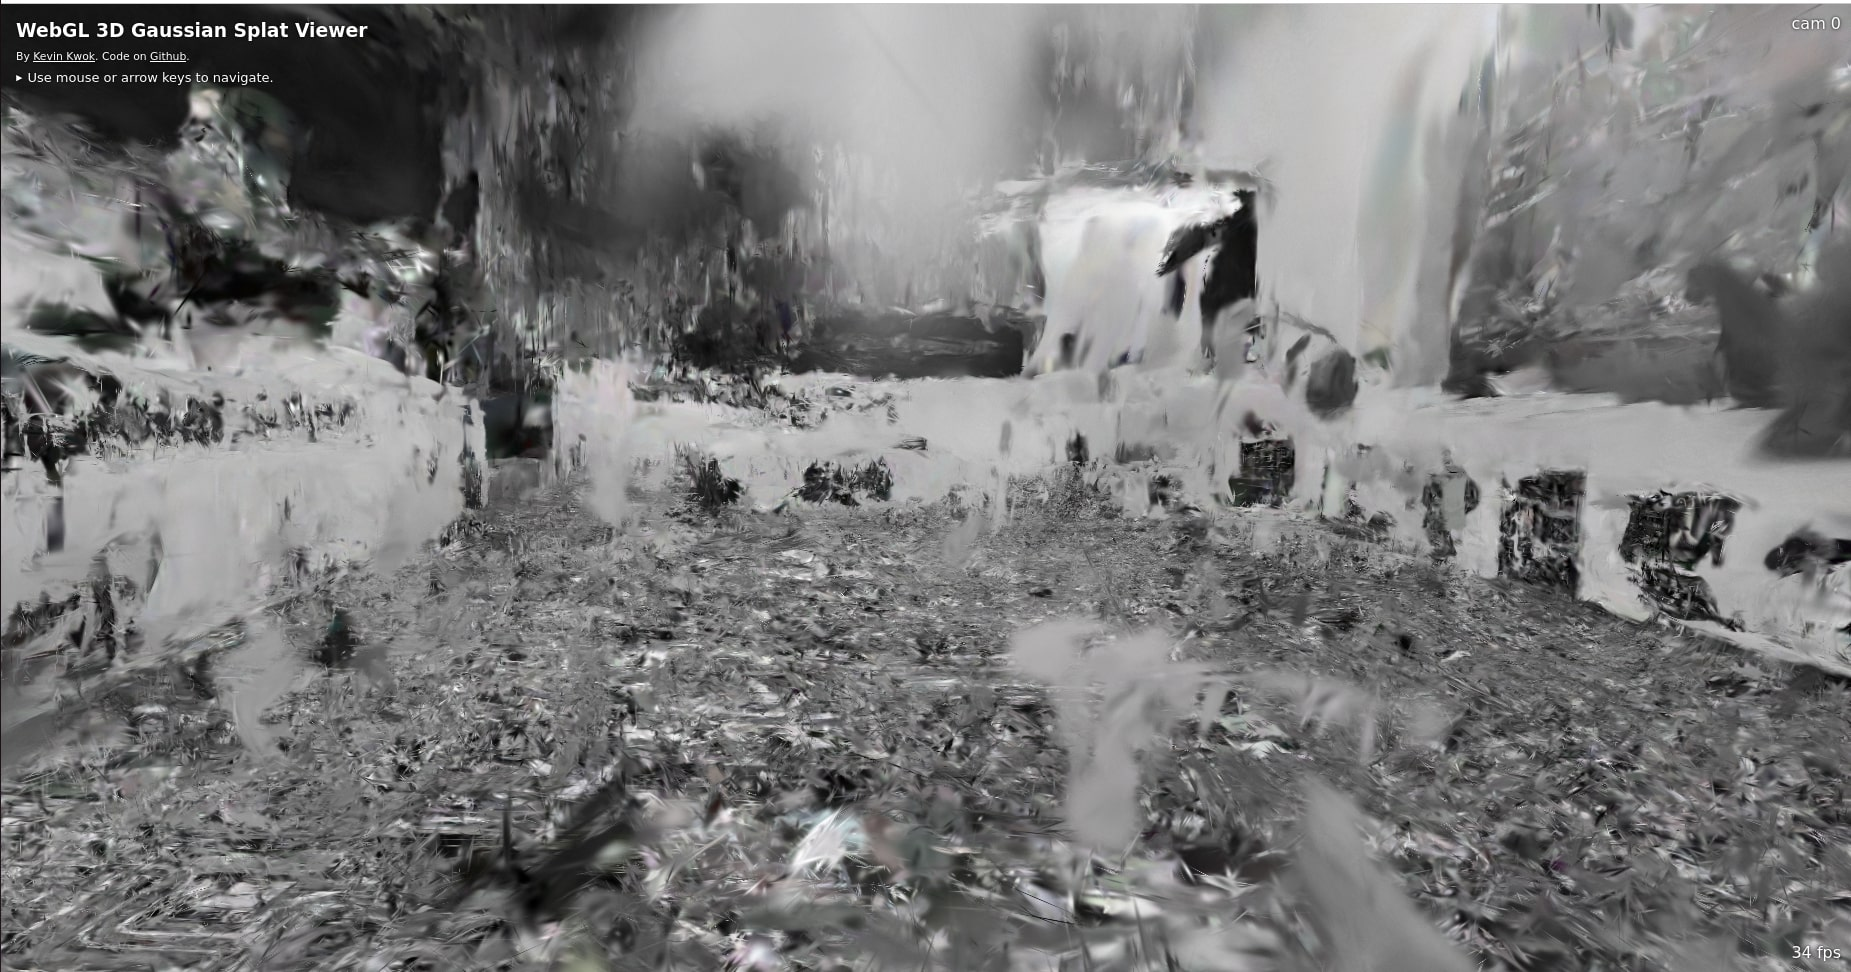
\includegraphics[width=150mm, keepaspectratio]{figures_jpg/nokia_splatfacto_ours1.jpg}
	\caption{Reconstructed map in the Nokia office with the \textit{splatfacto} model}
	\label{fig:nokia_splatfacto_ours_1}
\end{figure}

\begin{figure}[htbp]
	\centering
	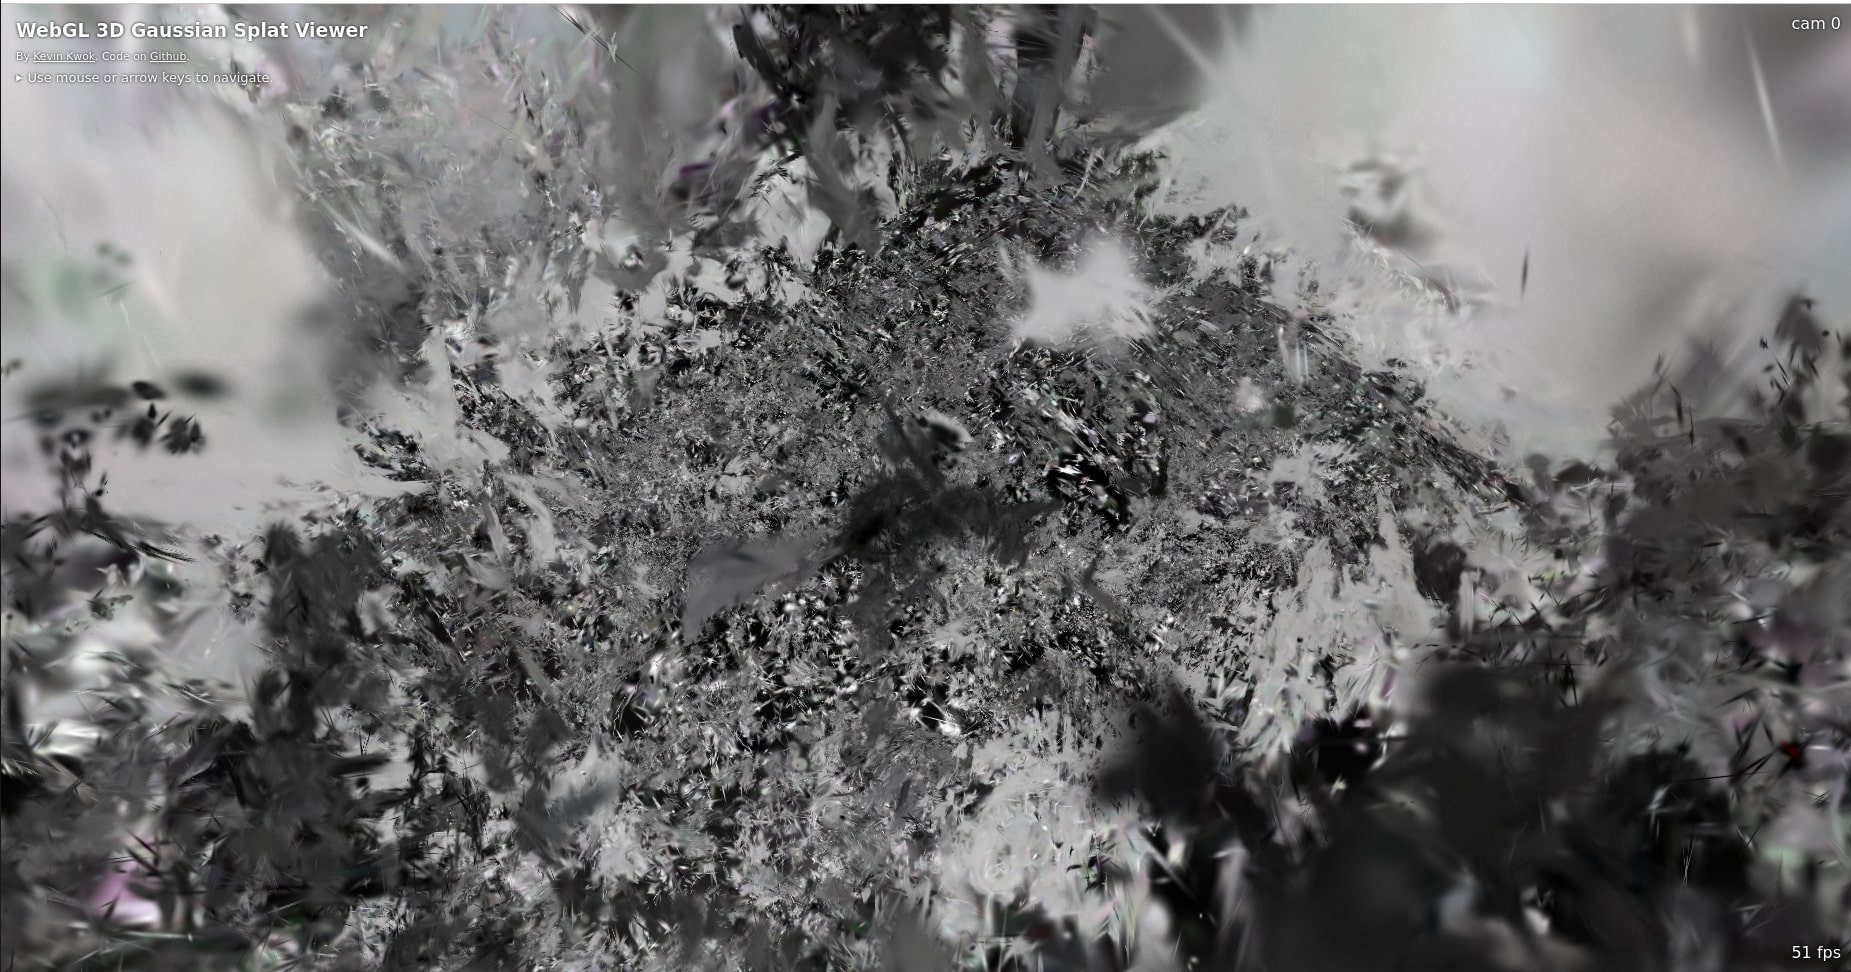
\includegraphics[width=150mm, keepaspectratio]{figures_jpg/nokia_splatfacto_ours2.jpg}
	\caption{Reconstructed map in the Nokia office with the \textit{splatfacto} model}
	\label{fig:nokia_splatfacto_ours_2}
\end{figure}

\begin{figure}[htbp]
	\centering
	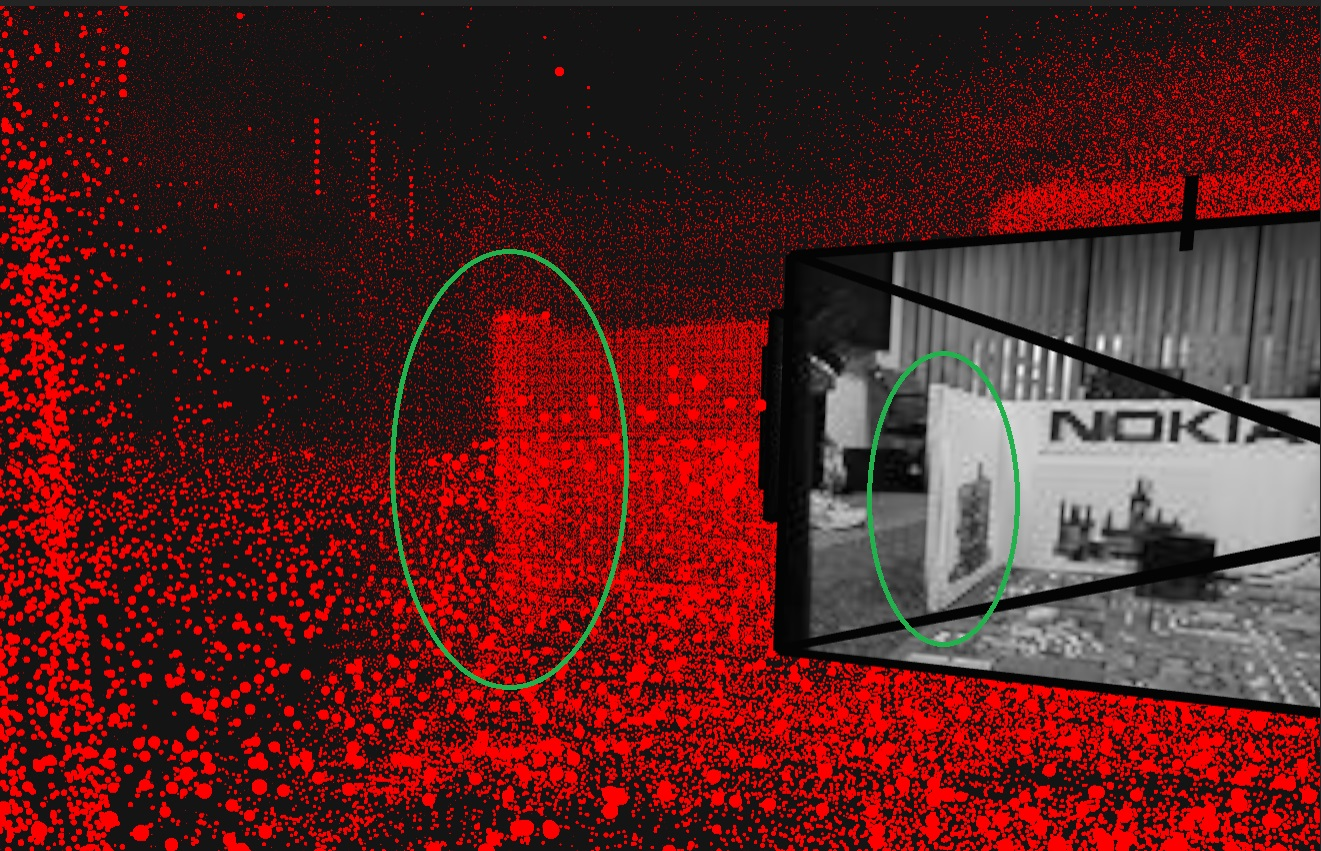
\includegraphics[width=150mm, keepaspectratio]{figures_jpg/trajectory_and_pointcloud_debug.jpg}
	\caption{Reconstructed map in the Nokia office with the \textit{splatfacto} model}
	\label{fig:trajectory_and_pointcloud}
\end{figure}

\begin{figure}[htbp]
	\centering
	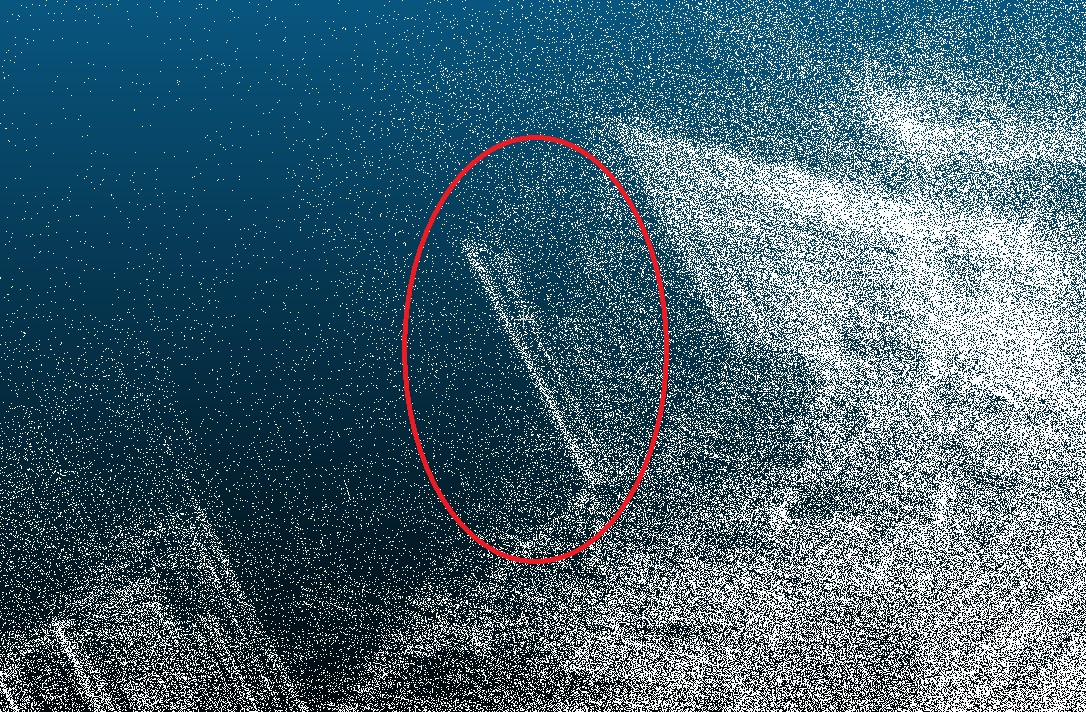
\includegraphics[width=150mm, keepaspectratio]{figures_jpg/pointcloud_debug.jpg}
	\caption{Reconstructed map in the Nokia office with the \textit{splatfacto} model}
	\label{fig:pointcloud_debug}
\end{figure}

\begin{figure}[htbp]
	\centering
	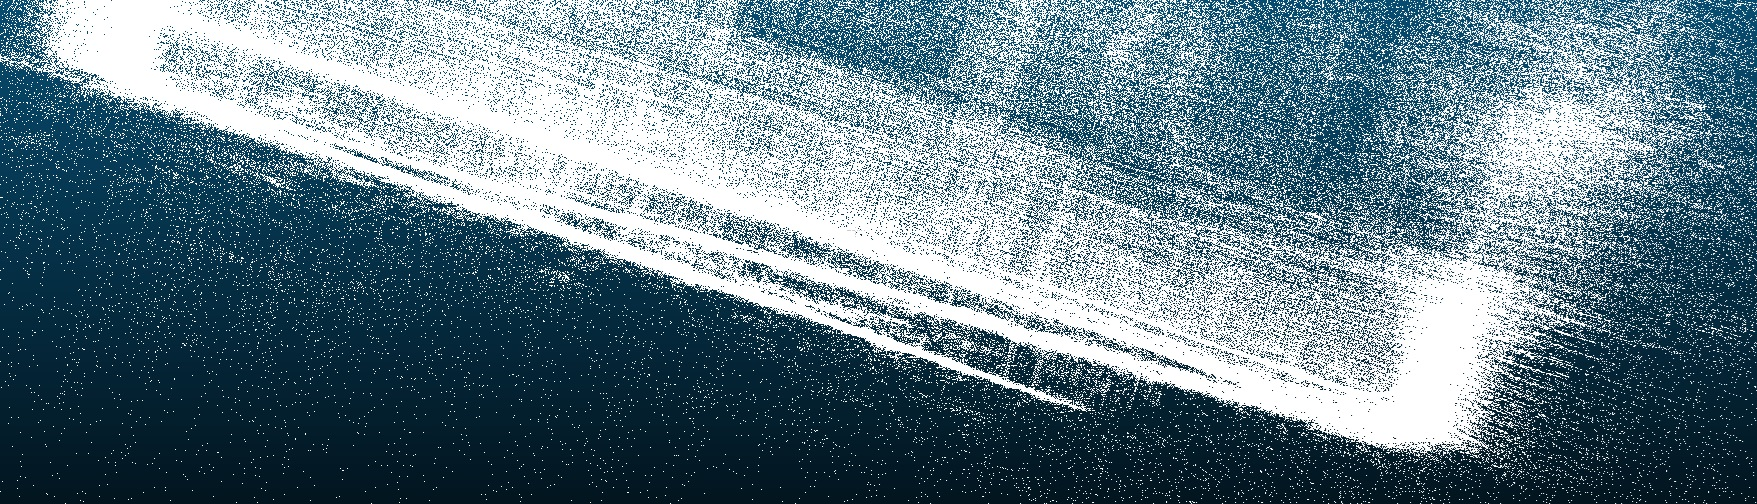
\includegraphics[width=150mm, keepaspectratio]{figures_jpg/pointcloud_debug1.jpg}
	\caption{Reconstructed map in the Nokia office with the \textit{splatfacto} model}
	\label{fig:pointcloud_debug1}
\end{figure}


To prove that the reconstruction can be used in mapping scenarios, we used the images with calculated poses and pointclouds to compare the results. For calculation we used COLMAP which can be used for pointcloud reconstruction and pose estimation from images. The result can be seen on Figure~\ref{fig:nokia_splatfacto_colmap_1} and Figure~\ref{fig:nokia_splatfacto_colmap_2}.
\begin{figure}[htbp]
	\centering
	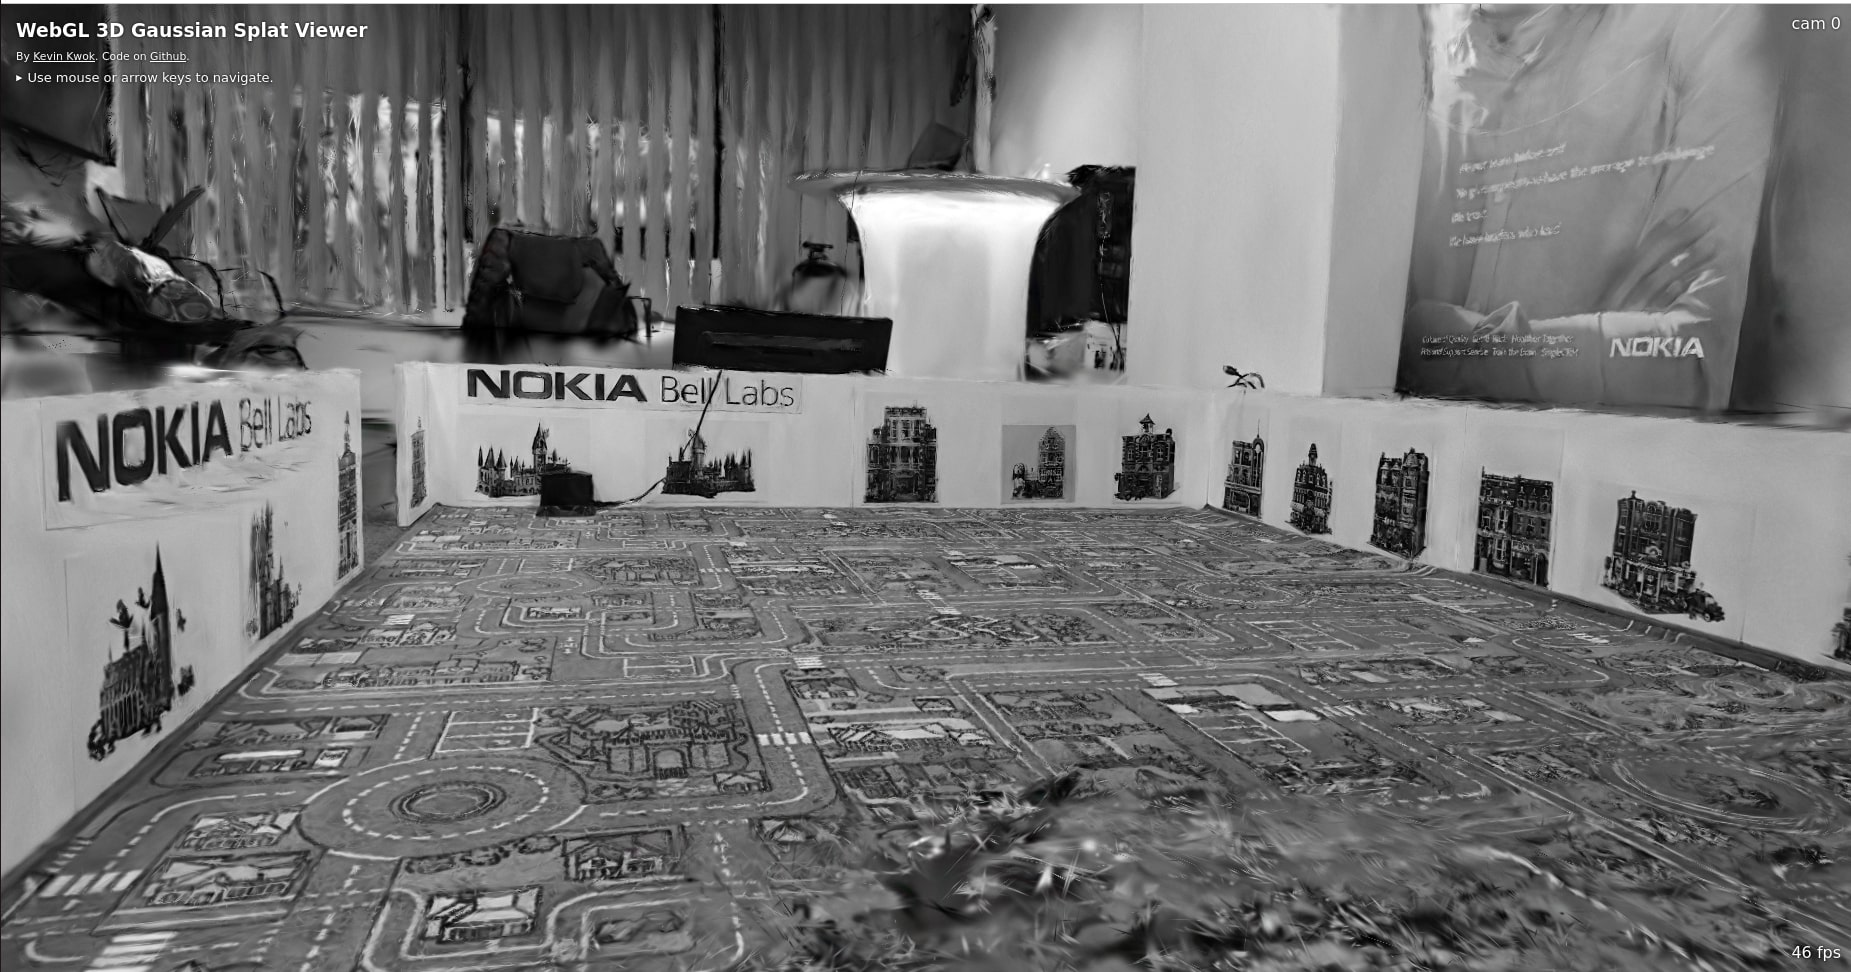
\includegraphics[width=150mm, keepaspectratio]{figures_jpg/nokia_splatfacto_1.jpg}
	\caption{Reconstructed map in the Nokia office with the \textit{splatfacto} model}
	\label{fig:nokia_splatfacto_colmap_1}
\end{figure}

\begin{figure}[htbp]
	\centering
	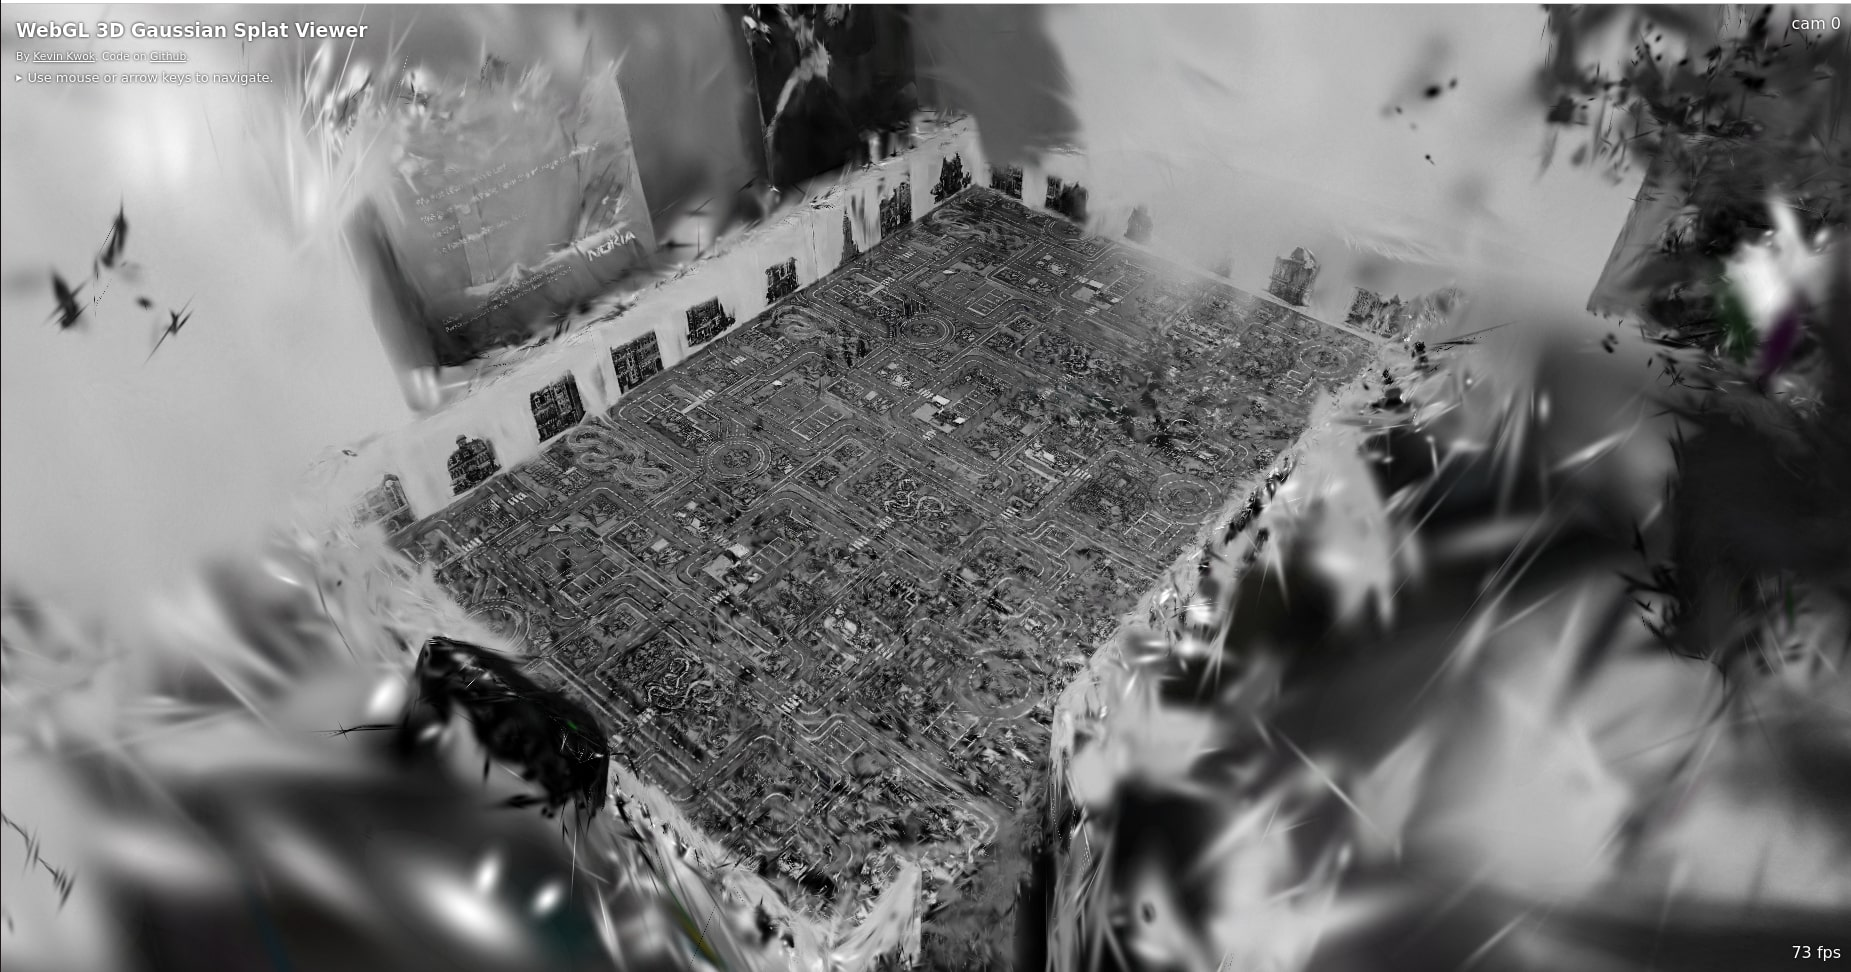
\includegraphics[width=150mm, keepaspectratio]{figures_jpg/nokia_splatfacto_2.jpg}
	\caption{Reconstructed map in the Nokia office with the \textit{splatfacto} model}
	\label{fig:nokia_splatfacto_colmap_2}
\end{figure}

In conclusion, it can be seen that the result where we used COLMAP for pose estimation and pointcloud reconstruction appears to depict the real environment precisely. If we would be able to somehow filter out the noise from the pointcloud calculated by the camera, our result would be as accurate as COLMAP's (or even more). Unfortunately we did not have time to implement this filtering during the thesis.
